\documentclass[11pt]{article}
\usepackage[utf8]{inputenc}
\usepackage{cs170}
\usepackage{derivative}
\usepackage{mathdots}

\def\title{}
\def\duedate{INSERT DUE DATE}


\begin{document}
\question{Median Filtering}

Recall that a convolutional kernel in image contexts involves calculating the sum of the elementwise products of the kernel with a window of pixels in the image, then sliding the kernel across the image, repeating the process for every pixel in the image.

\begin{subparts}
    \subpart Consider the following 3x3 kernel:
    $$\frac{1}{9} \begin{bmatrix}
    1 & 1 & 1 \\
    1 & 1 & 1 \\
    1 & 1 & 1
    \end{bmatrix}$$

    This is often referred to as a "box-blur" kernel. Why does it have a blurring effect?

    \answer{The box-blur kernel effectively averages each pixel with its neighbors. This means that the resulting image will be blurred, because sharp edges will become somewhat gradiented.}

    \subpart Now consider a related technique, known as \emph{median filtering}. Here, for a given window of pixels, the center pixel is replaced with the median of the pixels in the window. This process is then repeated across the entire image, just as is done with convolution.
    
    For your curiosity, depicted below are the results of applying 3x3 filters to an image (original left, box-blur center, median right):
    \begin{figure}[h] \centering
        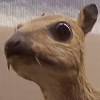
\includegraphics[width=0.3\textwidth]{orig.png}
        
\includegraphics[width=0.3\textwidth]{box_blur.png}
        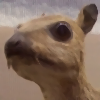
\includegraphics[width=0.3\textwidth]{median_filtered.png}
    \end{figure}

    Can you think of a scenario where median filtering would be preferable to box-blur filtering? What about the other way around?

    \answer{Median filtering can be very useful for denoising, especially where the noise is extremely pronounced, because it eliminates outliers, whereas box-blur filtering will be largely affected by outliers. Box-blur filtering is useful for universally blurring images, and is also easier to compute.}

    \subpart For ConvNets, are median filters similar to convolutional layers? Are they still useful? Why or why not?

    \answer{Median filters are not similar to convolutional layers, because they do not have learnable parameters. In this sense, they are more similar to pooling layers. However, they can certainly still be useful, e.g. in preprocessing steps, because of their denoising capabilities.}

    \subpart Consider the infinite zero matrix 
    $$\mathbf{0} = \begin{bmatrix}
        \ddots & \vdots & \vdots & \iddots \\
        \cdots & 0 & 0 & \cdots \\
        \cdots & 0 & 0 & \cdots \\
        \iddots & \vdots & \vdots & \ddots
    \end{bmatrix},$$ which, for this problem, represents a bitmap of constant color. Now suppose each pixel in the image is independently flipped to $1$ with probability $p < 0.2$, representing random noise. What is the expected result of applying a $3 \times 3$ box-blur filter to this newly noised image? What about a $3 \times 3$ median filter? Assume the stride length is at least 2.
    
    Do your answers to (b) and (c) now change?

    \answer{
        The expectation of the noise is $p$ times the all-ones matrix (denoted $\mathbf{J}$), and a box-blur filter simply averages all the pixels in its window, so the expected result of applying a box-blur filter is
        $$\frac{1}{9} \left( \mathbf{0} + p \cdot \mathbf{J} \right) = \frac{p}{9} \cdot \mathbf{J}.$$

        With a median filter, for a pixel to change, $1$ must be the new median of the window after the noise is applied, which means that at least 5 pixels must be flipped to $1$ in any given $3 \times 3$ window. The probability $q$ of this occurring is 
        \begin{align*}
            q := &\sum_{k=5}^9 \left(\begin{array}{c} 9 \\ k \end{array}\right) p^k (1-p)^{9-k} \\ 
            = \: &p^9 + 9 (1 - p) p^8 + 36 (1 - p)^2 p^7 + 84 (1 - p)^3 p^6 + 126 (1 - p)^4 p^5.
        \end{align*}

        The expected result of applying the median filter is then
        $$ \left( \mathbf{0} + q \cdot \mathbf{J} \right) = q \cdot \mathbf{J}.$$
        
        $q < \frac{p}{9}$, so if the goal is to restore the original image, median filtering performs much better at this sort of denoising task than box-blur filtering.
    }
    \subpart Let $K \times K$ denote filter size, $P$ padding size, $S$ stride length, and suppose we are operating on an image of size $H \times W$. What is the runtime complexity of convolution? How about median filtering? Assume no results are cached across different pixels.

    \emph{Hint: You can find the median of $n$ numbers in $O(n)$ time.}

    \answer{The image after padding is effectively $(H + 2P) \times (W + 2P)$. Stride reduces computation by approximately $1/{S^2}$, because each $S \times S$ window has only one elementwise product operation. For each pixel considered, there are $K^2$ multiplications. Thus, the complexity of convolution is $O(\frac{K^2}{S^2}(H + P)(W + P))$. However, padding is always less than the size of the image, so the complexity is $O(\frac{K^2 HW}{S^2})$. The complexity of median filtering is the same, because both the mean and the median take linear time to compute.}

\end{subparts}

\newpage

\question{Weighted Cross-Entropy}
	Recall that cross-entropy loss is given by
    $$
    \mathcal{L}(y, \hat{y}) = - y \log \hat{y} - (1 - y) \log (1 - \hat{y}),
    $$
    where $y$ is the ground truth label and $\hat{y}$ is the predicted probability that the label is $1$.

    \begin{subparts}
        \subpart Suppose $p$ is the ground-truth probability of a positive sample. Find the value of $\hat{y}$ that minimizes the expected loss
        $$\mathbf{E}_{y \sim \text{Bernoulli}(p)}\left[\mathcal{L}(y, \hat{y})\right]$$ by taking the derivative with respect to $\hat{y}$ and setting it to zero.

        \answer{The derivative is given by
            \begin{align*}
                \pdv{}{\hat{y}}\mathbf{E}_{y \sim \text{Bernoulli}(p)}\left[\mathcal{L}(y, \hat{y})\right] &= 0 \\
                \pdv{}{\hat{y}} (- p \log \hat{y} - (1 - p) \log (1 - \hat{y})) &= 0 \\
                - \frac{p}{\hat{y}} + \frac{1 - p}{1 - \hat{y}} &= 0 \\
                \frac{1 - p}{1 - \hat{y}} &= \frac{p}{\hat{y}} \\
                \hat{y}(1 - p) &= p(1 - \hat{y}) \\
                \hat{y} - p \hat{y} &= p - p \hat{y} \\
                \hat{y} &= p.
            \end{align*}
        }

        \subpart Now, consider how the model is affected by $p$. Find 
        $$\pdv{}{p} \mathbf{E}_{y \sim \text{Bernoulli}(p)}[\mathcal{L}(y, \hat{y})]$$
        using the minimizing value of $\hat{y}$ found in the previous subpart. From this, what values of $p$ will be problematic for our model's predictions from a convergence perspective? (You do not need to show this rigorously.)

        \answer{
            \begin{align*}
                \pdv{}{p} \mathbf{E}_{y \sim \text{Bernoulli}(p)}[\mathcal{L}(y, \hat{y})]
                &= \pdv{}{p} \left(- p \log \hat{y} - (1 - p) \log (1 - \hat{y})\right) \\
                &= - \log \hat{y} + \log(1 - \hat{y}) \\
                &= \log \frac{1 - \hat{y}}{\hat{y}} \\
                &= \log \frac{1 - p}{p}.
            \end{align*}
            When $\hat{y}$ is close to $0$ or $1$, the loss becomes very unstable. This is the case when $p$ is close to $0$ or $1$, indicating an unbalanced distribution. This means that we will need to have an extremely small learning rate to ensure convergence, which will slow training significantly.
        }

        \subpart Suppose we want to modify the loss function to be more robust to unbalanced distributions. One way to do this is to introduce a hyperparameter $\alpha$, which we can use to penalize incorrect predictions more heavily for the minority class (or equivalently, less heavily for the majority class). This is called \emph{weighted cross-entropy} and is given by
        $$
        \mathcal{L}_\alpha(y, \hat{y}) = - \alpha y \log \hat{y} - (1 - y) \log (1 - \hat{y}).
        $$
        \begin{enumerate}
            \item[(i)] Find the value of $\hat{y}$ that minimizes the expectation of this loss. Remember that the ground-truth probability of a positive sample is $p$, and $y \sim \text{Bernoulli}(p)$.
            
            \answer{Similarly to before, we take the derivative and set it to zero.
                \begin{align*}
                    \pdv{}{\hat{y}} \mathcal{L}_\alpha(y, \hat{y}) &= 0 \\
                    \pdv{}{\hat{y}} (- \alpha p \log \hat{y} - (1 - p) \log (1 - \hat{y})) &= 0 \\
                    - \frac{\alpha p}{\hat{y}} + \frac{1 - p}{1 - \hat{y}} &= 0 \\
                    \frac{1 - p}{1 - \hat{y}} &= \frac{\alpha p}{\hat{y}} \\
                    \hat{y}(1 - p) &= \alpha p(1 - \hat{y}) \\
                    \hat{y} - p \hat{y} &= \alpha p - \alpha p \hat{y} \\
                    (1 - p + \alpha p) \hat{y} &= \alpha p \\
                    \hat{y} &= \frac{\alpha p}{1 - p + \alpha p} \\
                \end{align*}
            }
            
            \item[(ii)] Use the value of $\hat{y}$ from part (i) to find $\alpha$ in terms of $p$ such that, when averaged over sufficiently many samples, both the minority and majority classes contribute to the total loss equally.
            
            \emph{Note: This derivation is quite difficult, but the final answer should be relatively simple. Feel free to use a symbolic or graphing calculator.}
            
            \answer{We want the loss to be equal for both the positive and negative classes, so we set
                \begin{align*}
                    % \mathcal{L}_{\text{batch}} &= \frac{1}{N} \sum_{i = 1}^N \mathcal{L}_\alpha(y, \hat{y}) \\
                    % &= \frac{1}{N} \sum_{i = 1}^N \left(- \alpha y \log \hat{y} - (1 - y) \log (1 - \hat{y})\right) \\
                    % \mathbf{E}[\mathcal{L}_{\text{batch}}] &= \frac{1}{N} \sum_{i = 1}^N \left(- \alpha p \log \hat{y} - (1 - p) \log (1 - \hat{y})\right) \\
                    % &= - \alpha p \log \hat{y} - (1 - p) \log (1 - \hat{y}) \\
                    \alpha p \log \hat{y} &= (1 - p) \log (1 - \hat{y}) \\
                    \alpha p \log \left(\frac{\alpha p}{1 - p + \alpha p}\right) &= (1 - p) \log \left(1 - \frac{\alpha p}{1 - p + \alpha p}\right) \\
                    \alpha p \log \left(\frac{\alpha p}{1 - p + \alpha p}\right) &= (1 - p) \log \left(1 - \frac{(1 - p + \alpha p) - (1 - p)}{1 - p + \alpha p}\right) \\
                    \alpha p \log \left(\frac{\alpha p}{1 - p + \alpha p}\right) &= (1 - p) \log \left(\frac{1 - p}{1 - p + \alpha p}\right) \\
                    \alpha p \left( \log(\alpha p) - \log(1 - p + \alpha p) \right) &= (1 - p) \left( \log(1 - p) - \log(1 - p + \alpha p) \right) \\
                    \alpha p \log (\alpha p) - \alpha p \log (1 - p + \alpha p) &= (1 - p) \log(1 - p) - (1 - p) \log(1 - p + \alpha p) \\
                    (1 - p - \alpha p) \log (1 - p + \alpha p) &= (1 - p) \log(1 - p) - \alpha p \log(\alpha p)
                \end{align*}
                Let $q = 1 - p$, then $p = 1 - q$, so
                \begin{align*}
                    (q - \alpha (1 - q)) \log (q + \alpha (1 - q)) &= q \log q - \alpha (1 - q) \log(\alpha (1 - q))
                \end{align*}
                Then let $r = \alpha (1 - q)$, so
                \begin{align*}
                    (q - r) \log (q + r) &= q \log q - r \log r
                    % (q - r) \log (q + r) &= \log(q^q) - \log(r^r) \\
                    % (q - r) \log (q + r) &= \log(\frac{q^q}{r^r}) \\
                    % e^{(q - r) \log (q + r)} &= \frac{q^q}{r^r} \\
                    % (q + r)^{(q - r)} &= \frac{q^q}{r^r} \\
                \end{align*}
                Note that the equation is invariant to swapping $q$ and $r$. This can be seen as follows:
                \begin{align*}
                    (q - r) \log (q + r) &= q \log q - r \log r \\
                    (r - q) \log (r + q) = -(q - r) \log (q + r) &= - (q \log q - r \log r) = r \log r - q \log q
                \end{align*}
                This suggests a symmetry over $q = r$, and indeed, it can be verified that $q = r$ satisfies the equation. This yields $q = r$ and we can solve for $\alpha$:
                \begin{align*}
                    q &= r \\
                    q &= \alpha (1 - q) \\
                    \alpha &= \frac{q}{1 - q} \\
                    \alpha &= \frac{1 - p}{p}
                \end{align*}
            }
        \end{enumerate}
        

        

    \end{subparts}

\end{document}
